\section{Example application HDL modules}
\label{sec:ExampleApp}
The example application, the user application inside the FPGA, replaces the counter with a pseudo-random data generator. Moreover the new feature in the application has the possibility to process data from the PC memory. A more detailed report about the example application can be found in \cite{ExampleApplication}

The example application can be operated in two modes:

\begin{enumerate}
	\item The random data generator directly sends data to the host via Wupper, this is referred to as "write only" or "half loop" test. 
	\item The content of the random data generator is wrote back to the FPGA, multiplied and sent to host again, this is referred as "read and write" or "full loop" test.  
	
\end{enumerate}

The example application is developed in VHDL, and the code is synthesized and implemented in Xilinx Vivado 2015.4~\cite{vivadoman}. The example application is now part of the Wupper package on OpenCores. 

\subsection {Functional blocks}

Figure~\ref{fig:benchmarkapp} shows a detailed block diagram of the example application for Wupper. The Wupper core contains a list of addresses, this list is the register map. The values of the register map are implemented in the firmware as signals. The PC sees the signals as addresses. Wupper tools write values to these addresses which control the FPGA logic (see dashed lines in Figure~\ref{fig:benchmarkapp}).
%http://www.eetimes.com/document.asp?doc_id=1274550

\begin{figure}[h]
	\centering
	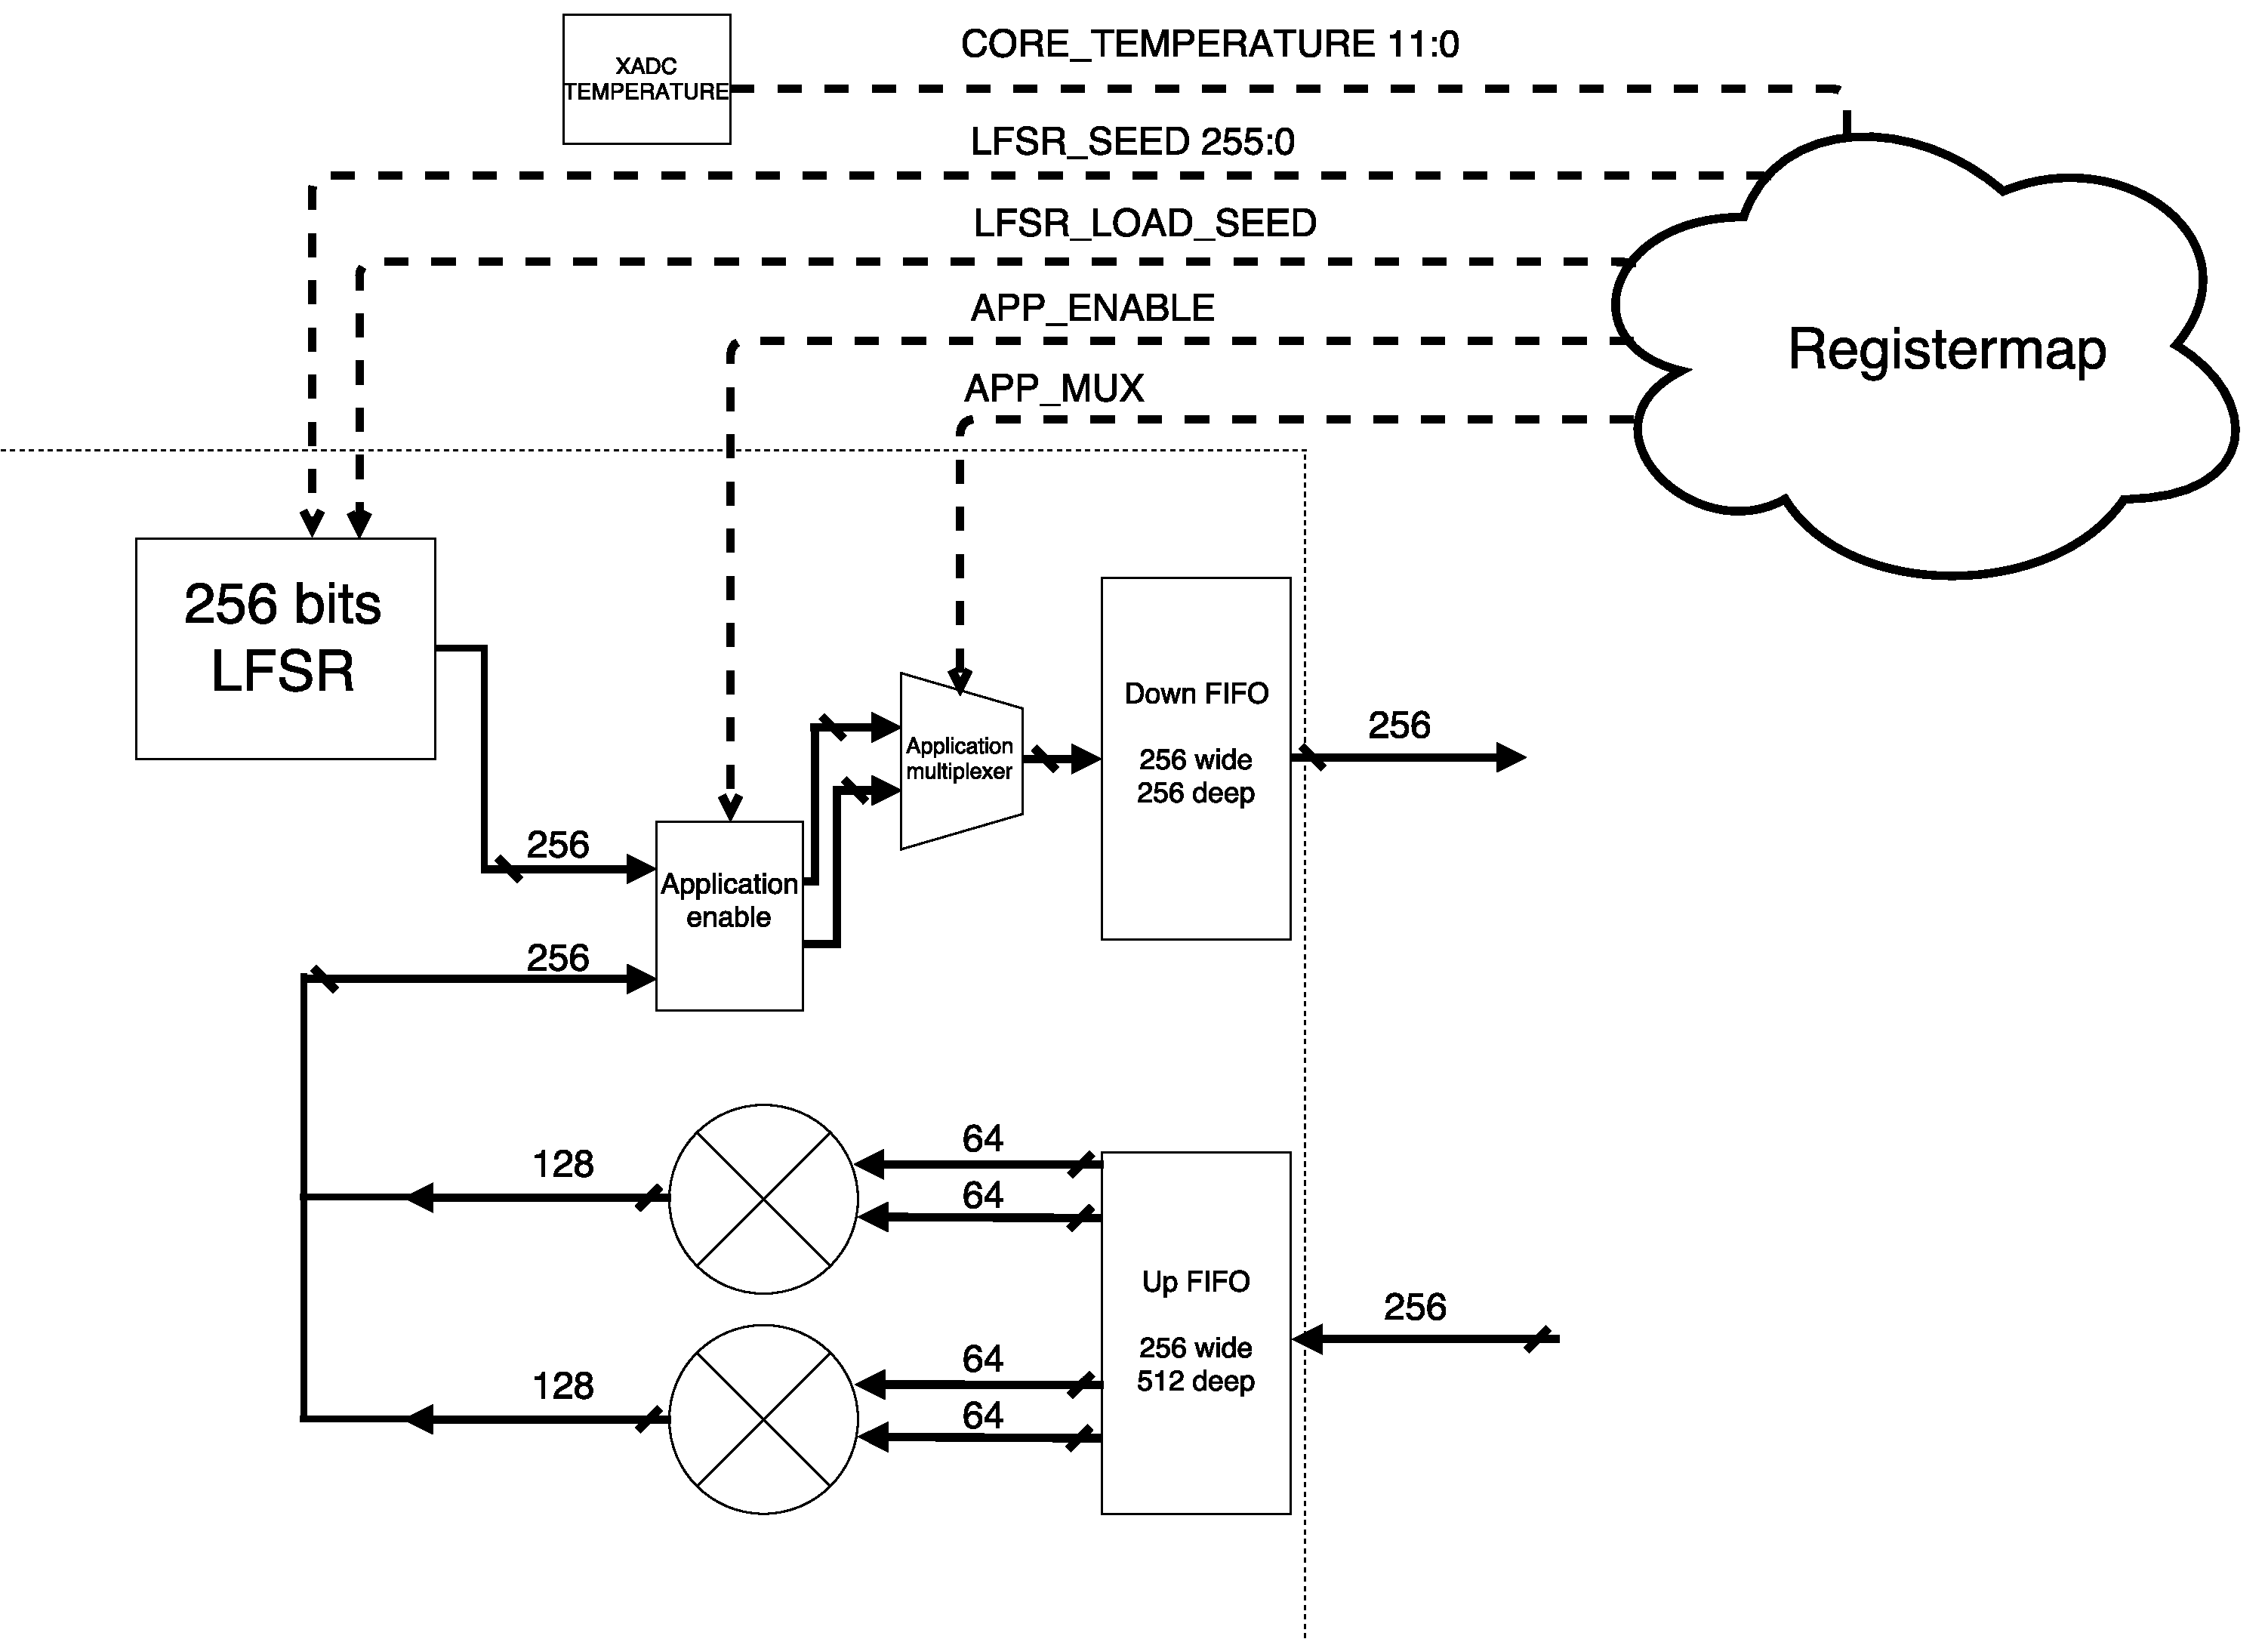
\includegraphics[width = 0.8 \textwidth]{figures/benchmark_application.pdf}	
	\caption{Overview of the example application}
	\label{fig:benchmarkapp}
\end{figure}

\newpage
As introduced in the previous paragraph, one type of test possible with the example application is the "half loop": in such mode of operation, Wupper is fed by a random data generator based on a 256 bits Linear Feedback Shift Register (LFSR). An LFSR, as shown in Figure~\ref{fig:lfsr}, consists of a number of shift registers which are fed back to the input. The feedback is manipulated by an XOR operation which creates a pseudo-random pattern. The ideal goal is to produce a sequence with a infinite length to prevent repetition. Repetition occurs by two factors, the feedback points/taps and the start value. The maximal length sequence can be approached by $2^n-1$~\cite{lfsr}. Where the $n$ is the number of shift registers. The 256 bits LFSR is a four stage Galois LFSR with taps at the registers 256, 254,251 and 246. The approach is explained in paper~\cite{lfsrtable} by R. W. Ward and T.C.A. Molteno of the electronics group at the University of Otago.
The software tools developed for the example application initialize the seed value by writing it to the register map thereafter the 1-bit $LFSR\_LOAD\_SEED$ signal is set to 1. This resets the LFSR process with a seed value.

\begin{figure}[H]
	\centering
	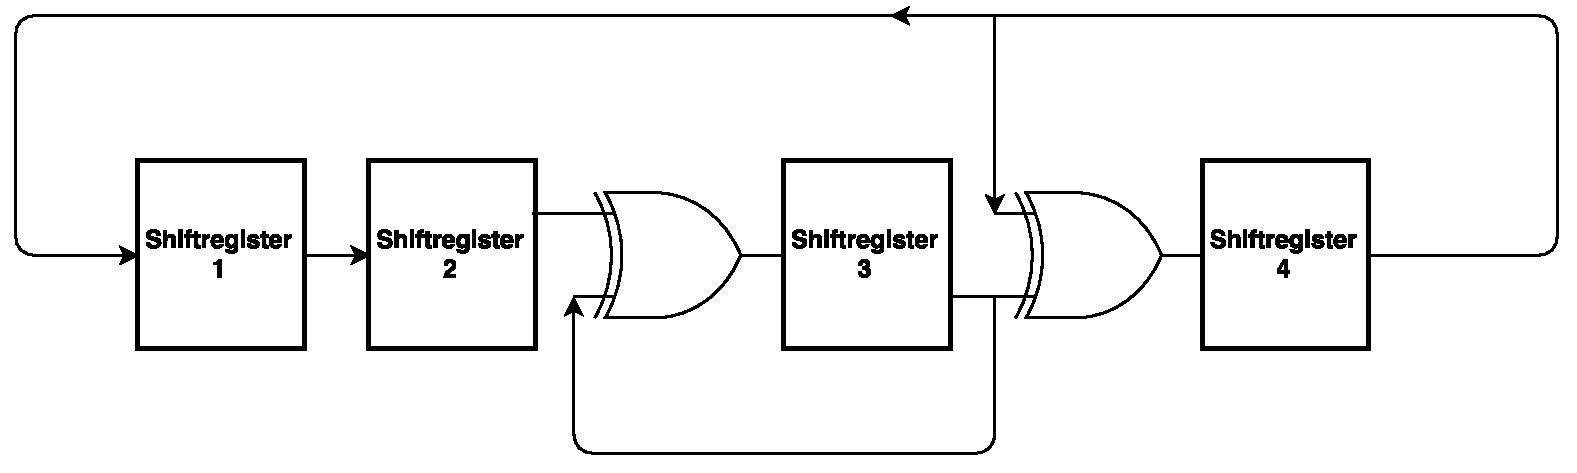
\includegraphics[width = 0.8 \textwidth]{figures/lfsr.pdf}	
	\caption{A 4 bit Linear Feedback Shift Register (LFSR)}
	\label{fig:lfsr}
\end{figure}
%http://www.newwaveinstruments.com/resources/articles/m_sequence_linear_feedback_shift_register_lfsr.htm
For multiplication, the Xilinx multiplier IP block is used. The operations are based on the DSP48E1~\cite{DSP84E1} for the Virtex-7 series. There are two parallel multipliers used with two unsigned 64-bit inputs. To make the multiplier perform optimally at high clock rates, an 18 stage pipelining is used.

For monitoring the core temperature, a XADC IP block~\cite{xadc} is used. This is generated by Vivado's XADC wizard. The output signal of the block is connected to one register of the register map.

The 1-bit signal $APP\_MUX$ is attached to the select port of the application multiplexer. This enables the data flow to the down FIFO.

The signal $APP\_ENABLE$ enables the output of the LFSR and the multiplier. The 2-bits signal has three states:
\begin{itemize}
	\item "00": No data flow, application is on standby.
	\item "01": Makes the example application enable 'high' causing data to flow only from the LFSR.
	\item "10": Makes the example application enable 'high' causing data to flow only from the multiplier.
\end{itemize}
The FIFO's are generated by Vivado's FIFO generator and using integrated common clock block RAMs. The clock is set to 250 MHz to reach the maximum theoretical throughput. The up FIFO is deeper to function as a buffer. This is an extra precaution. The reason is if the data is looped back in the application, both FIFO's can be full at the same time. If this occurs, the application stalls because of the loop back.

\newpage